\documentclass[8pt]{extarticle}

\usepackage[utf8]{inputenc}
\usepackage{multicol}
\usepackage[margin=0.5in]{geometry}
\usepackage{graphicx}
\graphicspath{ {./assets/img/} }

\title{Data 100 Final Exam Reference Sheets}
\author{Yuyang Zhong}
\date{May 16, 2019}

\twocolumn
\begin{document}

\section*{Data 100 Spring 2019 Final Exam Reference}

\subsection*{Sampling}
\subsubsection*{Simple Random Sample (SRS)}
Prob. of 1 in sample of k from population of n:
$$ P = \frac{k}{n} = \frac{1}{n} + \frac{1}{n-1} + \frac{1}{n-2} + ... + \frac{1}{n-k+1}  $$
Prob. of 1 from k samples selected from n:
$$ P= \frac{{n-1\choose k-1}}{{n\choose k}} $$

\subsubsection*{Cluster Sample}
Divide population into cluster, SRS to select cluster(s)

Prob. of 1 in sample = prob of 1's cluster in sample of k cluster from pop
$$ P =\frac{k\mbox{ clusters}}{n\mbox{ clusters of population}} $$


\subsubsection*{Stratified Sample}
Split into strata, SRS in \textbf{EACH} stratum

Prob of 1 in sample = prob of 1 selected from strata of n 
$$ P = \frac{1}{n} \mbox{, where } n = \mbox{strata size} $$

\subsubsection*{Multi-Stage}
Conditional event, SRS to select group, SRS to sample within selected groups
$$ P(Stage 2 | Stage 1) $$
\hline

\subsection*{Pandas}
\begin{verbatim}
#Data Frames
df.loc[row, col] #row/column names
df.loc[[name1, name2]] -> dataframe
df.loc[name1] -> series
df.iloc[row, col] #row/column indices

#Series
s.value_count() # unique value counts

grouped = df.groupby(by)
        
#Aggregate groupby object
        grouped.agg(func)
        func: max, min, fisrt, last, head
                (lambda sf: ...) 
                # manipulate subframe
                
#Filtering groupby object
        grouped.filter(func)
        func: (lambda sf: ...) 
        # filtering condition

#merge
        df1.merge(df2, left_on=, right_on=)
\end{verbatim}
\hline

\subsection*{SQL}
\subsubsection*{Basic Syntax}
\begin{verbatim}
SELECT  <columns>
FROM <relations(s)/tables>
[<join type> JOIN <relation/table>] 
[ON <predicate>]
[WHERE <predicate>]
[GROUP BY <column(s)>] [HAVING <predicate>]
[ORDER BY <column(s)>] [LIMIT <number>]

ORDER BY RANDOM LIMIT # = random sample
\end{verbatim}

\subsubsection*{Joins}
Returns NULL if not found\par
INNER: Intersection\par
LEFT OUTER: keep rows on left\par
RIGHT OUTER: keep rows on right\par
WHOLE OUTER: everything\par


\subsubsection*{CASE Statement}
\begin{verbatim}
CASE WHEN <predicate> THEN <rv_pred> 
     ELSE <rv_else>
     END
\end{verbatim}
\hline

\subsection*{RegEx}
\subsubsection*{Characters}
\begin{verbatim}
\d: Digits [0-9]
\w: Alphanumeric [a-zA-Z0-9]
\s: White space
\D,\W,\S: Inverses of respective groups
. : any character
\ : escape to match literals
\end{verbatim}

\subsubsection*{Quantifiers}
\begin{verbatim}
* : 0 or more times
+ : 1 or more times
? : exactly 0 or 1 times
{m} : exactly m times
{m, n} : between m to n times
{m, } : at least m times
{ , n} : at most n times
\end{verbatim}

\subsubsection*{Anchors}
\begin{verbatim}
^ : beginning of line
$ : end of line
\end{verbatim}

\subsubsection*{Grouping}
\begin{verbatim}
(...) : match all characters in capturing group
[^...] : excludes all specified
\end{verbatim}

\subsubsection*{In Python}
\begin{verbatim}
import re
re.match(pattern, string) # 1 match from beginning
re.search(pattern, string) # 1 match anywhere
re.findall(pattern, string) # list of all matches
re.sub(pattern, repl, string) # replace patterns
re.split(pattern, string) #split by pattern

s.str.extract(r'[group]') # extract by group
# will only return grouped regex match
\end{verbatim}
\hline

\subsection*{Kernel Density Estimation}
Smooth function to estimate probability distribution:

Center kernel at every point\par
add function together and take average\par
$\alpha$ : standard deviation of each kernel (large: spread apart, low/flat peak; small: centered, tall peak)\par

\subsubsection*{Gaussian}
$$ k_\alpha(x, z)=\frac{1}{\sqrt{2\pi\alpha^2}}e^{-\frac{(x-z)^2}{2\alpha^2}} $$
Decrease $\alpha$ decreases smoothness of plot.
\subsubsection*{Boxcar}
$$   \left\{
\begin{array}{ll}
      \frac{1}{\alpha} & -\frac{\alpha}{2} \leq x-z \leq  \frac{\alpha}{2}\\
      0 & \text{else} \\
\end{array}
\right. $$
Probability distribution area = 1\par
rectangle: $ \frac{1}{\alpha} \cdot \alpha $; bigger $\alpha$ more accurate\\
\hline

\subsection*{Dimensionality Reduction \& PCA with SVD}
Finding columns that are linearly independent in a design matrix (gives $Rank(X)$):
$$ X = \mathbf{u}\Sigma \mathbf{v^\top} $$
Where,

$X: n\times d$, normalized original dataset (“feature matrix”)\par
$\mathbf{u}: n\times r$, left singular vectors, orthonormal\par
$\Sigma: r\times r$, diagonal matrix of singular values. The $k$-th singular value is the sum of the squares of the projections of the points to the line determined by the $k$-th singular vector.\par
$\mathbf{v^\top}: r\times d$, right singular vectors, orthonormal\\

\textbf{Directions}

$\mathbf{v1}$ = the unit vector $\mathbf{v}$ that maximizes $|X\mathbf{v}|$\par
$\mathbf{v2}$ = the unit vector $\mathbf{v}$ that is orthogonal to $\mathbf{v1}$ and maximizes $|X\mathbf{v}|$\par
The $i$-th singular value of $X$, or $\sigma_i(X)$, is given by $|X\mathbf{v_i}|$. The first $k$ columns of $X\mathbf{v^\top}$ (or $\mathbf{u}\Sigma$) are the first $k$ principal components\\

\textbf{Computations}

1. Centering Matrix:
\begin{verbatim}
  n = X.shape[0]
  X_transformed = (X - np.mean(X, axis=0))/np.sqrt(n)
\end{verbatim}

2. Use SVD to find PCs:
\begin{verbatim}
  u, s, vt = np.linalg.svd(X_transformed, full_matrices=False)
\end{verbatim}

3. Selecting PCs
\begin{verbatim}
  (u * s)[:,0]        X @ vt[0,:]         (X @ vt.T)[:,0]
\end{verbatim}
\hline

\subsection*{Visualizations}
\textbf{Things to Consider}

Granularity: what each row represents\par
Faithfulness: does data accurately capture reality\par
Temporality: how does data situate in date/time\par
Scope: coverage of data in relations to analysis (completeness) \\


\textbf{Plots}

Single Discrete: dot plot/bar plot\par
Single Continuous: strip plot (small), density plot/bar plot (big) \par
Multiple Continuous: Scatter plot\par
Discrete vs. Continuous: Box plot, overlay density plot, violin plot\par
2 Discrete vs. 2 Continuous: Sub-scatter, color, symbols, overlays\\

\hline

\subsection*{Probability, Expectations \& Variance}
\subsubsection*{Sampling}
Without replacement = ${n \choose r} = {_nC_r} = \frac{n!}{n!(n-r)!}$ ways\par
Prob of picking 1: $\frac{(n-1) {_nC_r}}{{_nC_r}}$ \par
With replacement = $n^r$ ways \par
Prob of picking 1: $1-\frac{(n-1)^r}{n^r}$ \par

\begin{multicols}{2}
[
\subsubsection*{Expectation}
]
$E[X]=\Sigma {(p(x_i)\cdot x_i)}$\par
$E[X+Y] = E[X] + E[Y]$\par
$E[cX] = c\cdot E[X]$\par
$E[XY] = E[X]\cdot E[Y]$ (indep.)\par
Median Absolute deviation: $Median[X-Median[X]]$\par
\end{multicols}

\subsubsection*{Variance}
$Var[X] = E[(X-E[X]^2] = E[X^2] - E[X]^2$\par
$Var[aX] = a^2 \cdot Var[X]$\par
$Var[X+Y] = Var[X] + Var[Y] + 2 Cov[X, Y]$\par
$Cov[X, Y] = Var[X] \cdot Var[Y] = E[XY] - E[X]\cdot E[Y]$\par

Same mean/variance $\neq$ same data

\subsubsection*{Bernoulli}
$E[X_i] = p$ and $Var[X_i]=p(1-p)$\par
Calculating variance: $Var[Y]=Var(\frac{1}{n}\sum{x_i})$\par
or, for Bernoulli: $Var[X]=np(1-p), y=\frac{1}{100}(x)$\par
\hline


\subsection*{Probability Distribution}
\subsubsection*{Gaussian}
$$ f_N(x:\mu, \sigma)=\frac{1}{\sqrt{2\pi\sigma^2}}e^{-\frac{(x-\mu)^2}{2\sigma^2}} $$
\subsubsection*{Bernoulli}
$$ f_{\mbox{binary}} (y:n, p) = {_nC_y} \cdot p^y(1-p)^{n-y} $$ 
\hline

\subsection*{Linear Algebra Properties}
\begin{multicols}{2}
$\mathbf{a}\cdot \mathbf{a} = \mathbf{a}^\top \mathbf{a}$\par
$\mathbf{a}\cdot \mathbf{b} = \mathbf{b}^\top \mathbf{a} = \mathbf{a}^\top \mathbf{b}$\par
$(AB)^\top = B^\top A^\top$ \par
$\nabla_x \mathbf{a}^\top \mathbf{x} = \nabla_x \mathbf{x}^\top \mathbf{a} =\mathbf{a} $ \par
$\nabla_x \mathbf{x}^\top A\mathbf{x} = (A+A^\top)\mathbf{x}$, $=2A\mathbf{x}$ if $A=A^\top$ symmetric 
\end{multicols}

Projection Matrix: $A^2 = A$ \\
\hline

\subsection*{Loss \& Risk Optimization}
\subsubsection*{Loss Functions}
Measuring loss at a specific point/observation:\par
$L_1 = |y-\hat{y}|$, minimized by median \par
$L_2 = (y-\hat{y})^2$, minimized by mean \par
Huber: $   \left\{
\begin{array}{ll}
      \frac{1}{2} (y-\hat{y})^2 &  |y-\hat{y}|\leq \alpha \\
      \alpha  |y-\hat{y}| - \frac{1}{2}\alpha & \text{else} \\
\end{array}
\right. $\par
\textbf{To find empirical risk, average loss from every point!}

Minimizing/estimating parameter: \begin{array}{ll}
      \mbox{Find Derivative of Risk} \\
      \textbf{($\beta$ is Constant!)}\\
      \mbox{Set Derivative to 0}\\
      \mbox{Solve for} $\beta$\\
\end{array} \\

\subsubsection*{Regularization, Bias \& Variance Trade-off}
Risk is the average loss over an entire set of observations: \par
Risk = $E[(\mathbf{y}-f(\mathbf{x}))^2] = (E[f(\mathbf{x})] - \mathbf{y})^2 + E[(f(\mathbf{x})-E[f(\mathbf{x})])^2] $\par
$= Bias^2[\mathbf{y}, f(\mathbf{x})] + Var[f(\mathbf{x})]$ \par
\begin{center}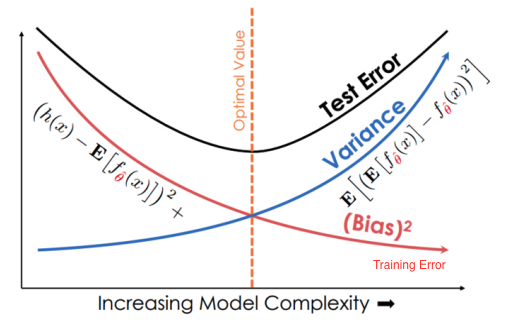
\includegraphics[width=0.33\textwidth]{b-v-tradeoff}\par \end{center}
Polynomial: higher degree, $Bias \downarrow, Variance \uparrow $, model complexity $\uparrow$\\

\textbf{Regularization for Mean Squared Error Function}\par
Regularize when \textbf{high loss, high variances}, controlling low bias

$\lambda \rightarrow 0,  \hat{\theta} \rightarrow L_2 $, little regularization\par
$\lambda \rightarrow \infty,  \beta_i \rightarrow 0 $, constant model, under-fit \par
$\lambda \uparrow \rightarrow Bias \uparrow \rightarrow Variance \downarrow $\\

\textbf{Ridge ($L_2$)}:$\frac{1}{n}\|{y-X\beta}\|_2^2 + \lambda \sum \beta^2$ \par
$\beta^* = (\mathbf{x}^\top \mathbf{x} - \lambda I)^{-1}\mathbf{x}^\top \mathbf{y}$\par
Distribute weight across related feature \par
Does not encourage sparsity \textbf{(does not set anything to 0)} \\
 
\textbf{LASSO ($L_1$)}: $\frac{1}{n}\|{y-X\beta}\|_2^2 + \lambda |\beta |$ \par
No Analytical Solution $\beta^*$ \par
Encourages sparsity \textbf{setting some weight to 0, decrease some} (feature selection) \\

\textbf{Linearity of features}: $x$ terms can be polynomial, but $\beta$ must be in separate terms and unique to each $x$. \par
\textbf{Convexity}: All lines connecting two points of the graph appear above the graph.\\
\hline

\subsection*{Linear Regression \& Least Squares}
\textbf{Linear Regression Model}: $E[Y|X]=X^\top \beta$ 

\textbf{Normal Equation}: \par
$L(\beta)=\mathbf{y}^\top \mathbf{y}-2\beta^\top \mathbf{x}^\top \mathbf{y}+\beta ^\top \mathbf{x}^\top \mathbf{x}\beta$ \par
$\nabla_\beta L(\beta)= \mathbf{x}^\top \mathbf{x}\beta -\mathbf{x}^\top\mathbf{y} = 0 $ \par
$\beta^* = (\mathbf{x}^\top \mathbf{x})^{-1}\mathbf{x}^\top \mathbf{y} = \sum^{n}_{i=1} \frac{x_iy_i}{x_i^2}$ \\

\textbf{Conditional Covariance}: \par
$Cov[\hat{\beta} | \mathbf{x}] = \sigma^2(\mathbf{x}^\top \mathbf{x})^{-1}$, where $Var[Y|X]=\sigma^2$ \par

\begin{center} 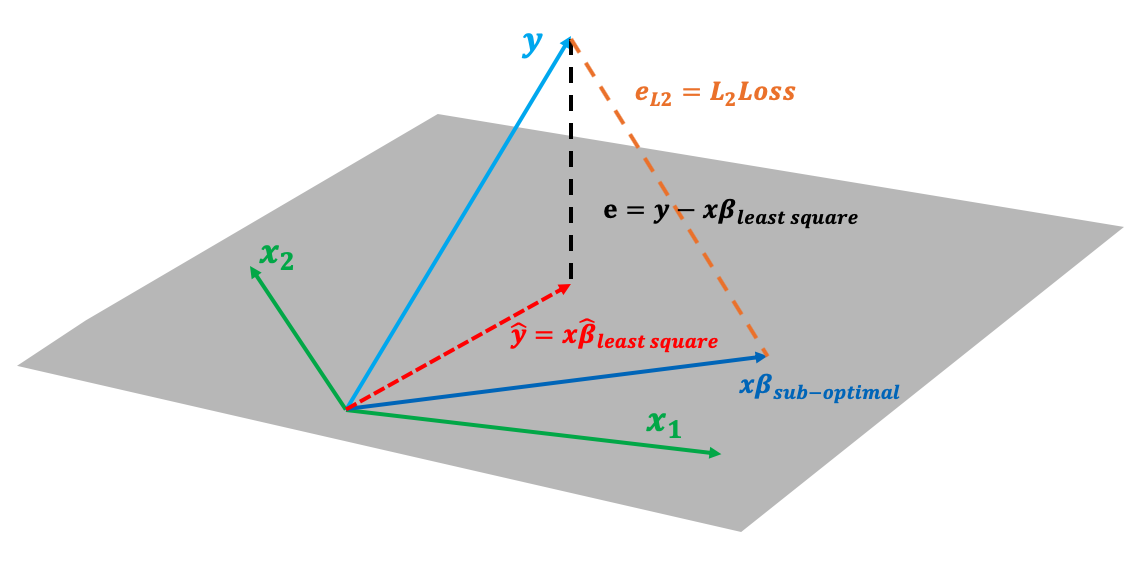
\includegraphics[width=0.45\textwidth]{leastsquares}\par \end{center}

*error/residuals need to be orthogonal to $Col(X)$ (aka MSE)\par
$X: n \times p$, to find some $\hat{\beta}$ that minimizes $\|e\|^2_2 $ \par
$\hat{\mathbf{y}}$ : observed $\mathbf{y}$ projected on $Col(X)$, linear, orthogonal to residuals \par
Sum of residuals = 0 \\
\hline

\subsection*{Gradient Descent}
$$\beta ^{t-1} = \beta^t-\alpha \nabla_\beta L(\beta^t)$$
$\alpha$ = learning rate\par
standard/batch: use all points \par
stochastic: pick random point to approximate batch \par
mini-batch: pick $k$ random points \\

\textbf{Algorithm}:
\begin{verbatim}
def grad_desc(x, y, theta, iter=#, alpha=#):
    for i in range(iter):
        grad = dt(x, t, theta)
        theta = theta - alpha * grad
        loss = mse(model(x, theta[0], theta[1], y))
        theta_history.append(theta)
        loss_history.append(loss)
    return theta, theta_history, loss_history
        
\end{verbatim}
\hline

\subsection*{Cross Validation}
Fold = \# of times splitting 

\textbf{Algorithm}:
\begin{verbatim}
def CV_error(model, X_train, Y_train):
    kf = KFold(n_splits = 4)
    validation_errors = []
    
    for train_idx, valid_idx in kf.split(X_train):
        # Split Data
        split_X_train = X_train.iloc[train_idx]
        split_X_valid = X_valid.iloc[valid_idx]
        split_Y_train = Y_train.iloc[train_idx]
        split_Y_valid = Y_valid.iloc[valid_idx]
        
        # Fit Model
        model.fit(split_X_train, split_Y_train)
        
        # Compute Error
        Y_pred = model.predict(split_X_valid)
        error = rmse(Y_pred, split_Y_valid)
        
        valifation_errors.append(error)
        
    return np.mean(validation_errors)

\end{verbatim}

\hline

\subsection*{Logistic Regression/Classification}
\textbf{Equations}:\par
\textbf{Logistic Regression Model}: $E[Y=1|X]=\sigma(X^\top \beta)$\par
$log(\frac{P(Y=1|X)}{P(Y=0|X)}) = X^\top \beta$ \par
The intercept term helps us shift the center/inflection point of the sigmoid away from the origin.\\

\textbf{Sigmoid Function}: $\sigma(t)= \frac{1}{1+e^{-t}} = \frac{e^t}{1+e^t}$ \par
$\sigma(-t) = 1-\sigma(t)$ \par
$\sigma'(t) = \sigma(t)(1-\sigma(t))$ \par
$X^\top \beta \rightarrow \infty, \sigma(t)\rightarrow 1$\par
$X^\top \beta \rightarrow -\infty, \sigma(t)\rightarrow 0$ \par

\subsubsection*{Cross Entropy Loss}
$-\mathbf{y_i}log(\theta) - (1-\mathbf{y_i})log(1-\theta)$ \\

TFAE when $\theta = \sigma(\mathbf{x_i^\top}\beta) $: \par
$L(y, \theta) =$ \par
$-\mathbf{y_i}log(\sigma(\mathbf{x_i^\top}\beta)) - (1-\mathbf{y_i})log(1-\sigma(\mathbf{x_i^\top}\beta))$ \par
$-\mathbf{y_i}\mathbf{x_i^\top}\beta +log(\sigma(-\mathbf{x_i^\top}\beta))$ \par

\subsubsection*{Classifier Evaluation}
\begin{center}
\begin{tabular}{ |c| c |c| } 
\hline
  & 1 & 0 \\ 
 \hline
 1 & TP & FP \\  
 \hline
 0 & FN & TN \\
 \hline
\end{tabular}
\end{center}

\textbf{accuracy}: (TP+TN)/n \par
\textbf{error}: (FP+FN)/n \par
\textbf{precision}: TP/(TP+FP) (\# of correct label over all true labels) \par
\textbf{recall}: TP/(TP/FN) (\# of true labels over all actually true items) \par

\textbf{Code}:
\begin{verbatim}
np.count_nonzero(
    (y==y_pred) & (y_pred==1)  #TP
    (y==y_pred) & (y_pred==0)  #TN
    (y!=y_pred) & (y_pred==1)  #FP
    (y!=y_pred) & (y_pred==0)  #FN
)
\end{verbatim}

\subsubsection*{Linear Separability}
$d$-dimensional points, draw a $d-1$ dimension line/plane to separate points:\par
\begin{center}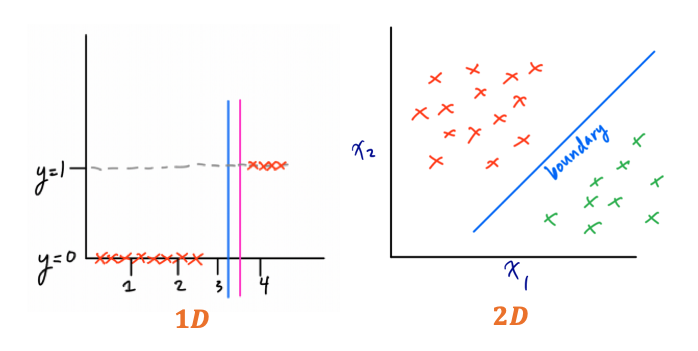
\includegraphics[width=0.4\textwidth]{separate}\par \end{center}
To be linearly separable, the data just needs to be separable on \textbf{one of the feature columns}. \par
* if data is linearly separable, then we can choose some $\beta$ such that the cross entropy loss $\rightarrow0$, and our optimal $\beta \rightarrow \infty$ (vertical line)  (OR: our $\beta$'s in the model will be very large, and will not be set to 0 by LASSO.) \textbf{Should regularize.}\\ 
\hline

\subsection*{Tree-Based Methods}
\subsubsection*{Decision Trees}
Each node represents a variable, and \textbf{splits based on variable’s values}. Leaf node associated with \textbf{prediction values} \par
Training: Identify how tree should be structured \par
Prediction: start from root, leaf node signifies prediction \\

1. Selecting splits; \par
2. Decide whether to declare node to be terminal or continue; \par
3. Assign fitted values at each terminal node

\subsubsection*{Deciding Splits}
Split at each node to maximize decrease in risk of current node (locally optimal) \par
Greedy Optimization: minimum risk occurs by taking a sub-optimal split at current node; depth first search computationally expensive \par
Classification: Impurity Measures as Risk Function (out of scope) \par
Regression: Squared Loss, Absolute Loss, Huber Loss \par

\subsubsection*{Stopping Splits + Prune to Avoid Overfitting}
To prevent overfitting and classify over every single point: \par
\textbf{Pruning}: remove section of tree that has little effect \par
Set \textbf{maximum tree depth}, \textbf{minimum number of samples} required to split, or \textbf{maximum impurity threshold}\\

\subsubsection*{Ensamble Methods}
Building multiple trees to avoid overfitting \par
Regression: average/median across tress (reduce variability + smooth regression surface)\par
Classification: majority vote \par
\textbf{Bagging (Bootstrap Aggregating)}: same tree trained on multiple bootstrap sample (good when single tree overfit)\par
\textbf{Boosting}: Assign higher weights to misclassified points (combined weak learners to create 1 strong learner)\par
Difference in Prob: Bagging - each point has equal chance of resample; Boosting - weights determined by performance \\

\subsubsection*{Pros \& Cons}
\begin{multicols}{2}
\textbf{Pros}: \par
Highly interpretable \par
Performs variable selections without LASSO \par
Works well with nonlinear boundaries\\

\textbf{Cons}:\par
Easy to overfit \par
Requires a lot of fine tuning \par
Outperformed by other ML techniques \\
\end{multicols}

\subsubsection*{Random Forest}
Build many trees using bootstrap samples (bagging)\par
When training each tree, at each node we take a sample of predictors and split\\
\hline

\subsection*{Bootstrapping}
\subsubsection*{Confidence Interval}
Finding Confidence Interval: \par
1. Sort collection in increasing order \par
2. Find $p\%$ (percentile) of $n$: $(p/ 100) \times n = k$ \par
3. If $k$ is an integer, take the $k$th element of the sorted collection \par
4. Else, round it up to the next integer, and take that element of the sorted collection. \\

\subsubsection*{Interpretation of CI}
Redraw $k$ sets of bootstrap samples, and calculate $k$ $\alpha \%$ Confidence Intervals, $\alpha \%$ of them will contain the true parameter of the \textbf{sampling population}. \\
\hline

\section*{Big Data}
\subsubsection*{Data Organization}
\textbf{Database & Data Warehouse}:\par
Data are extracted, transformed, and loaded \par

\textbf{Star schema}:
Fact table: contains \textbf{unique} primary keys + foreign key references to dimension tables\par
Dimension tables: primary keys are unique values to this dimension\par
\textbf{Snowflake schema} expands on each star to have dependent dimension tables and fact table. \\

\textbf{Data Lake - Unstructured Data}:
Store data in \textbf{raw form}\par
Requires knowledge in access/query \\

\subsubsection*{Distributed Computing}
Split one large file into parts, then distribute across multiple machines: \par
\textbf{Total fragments made} = \# of fragments * \# of replications \par
\textbf{Fragment/machine} = Total fragments made / \# of machines \par
\textbf{Maximum \# machine fail} = \# of replications - 1 \\

\subsubsection*{Map Reduce Model}
\begin{center}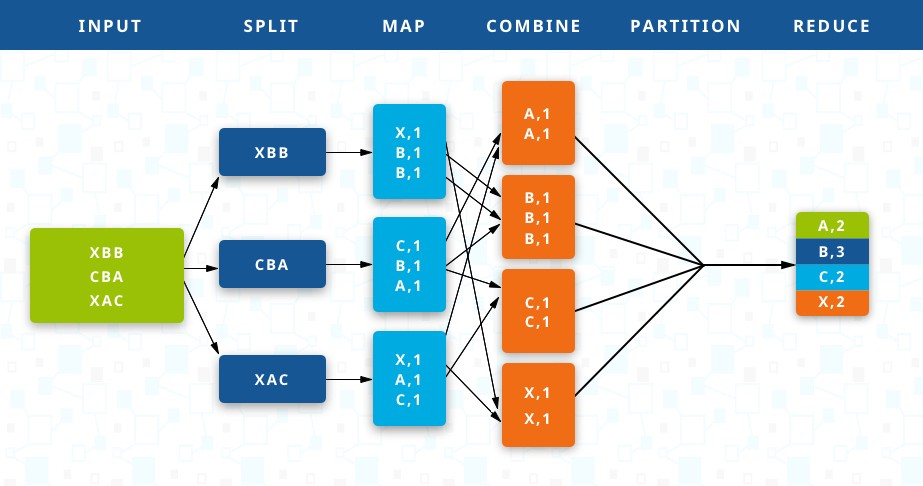
\includegraphics[width=0.45\textwidth]{mapreduce}\par \end{center}

\textbf{Map}: takes a dataset and a function and applies function on all points \par
\textbf{Reduce}: aggregates output of the map stage \par
*During reduce, all records associated to a given key are sent to the same machine.\par
*Reading from a large file from distributed machine is faster. \par

\subsubsection*{Ray}
Distributed execution engine, utilizes multiple CPU:\par
\textbf{Worker}: worker processes execute tasks \par
\textbf{Object Store}: immutable objects of processed task stored here, allow workers to efficiently share objects on the same node \par
\textbf{Task}: stateless function that can be execute on a remote server (functions) \par
\textbf{Actor}: stateful object that lives in a remote process (class/object-oriented) \par
*remote process returns object id, use ray.get() to get the actual values back \\
\hline

\end{document}
